\section{Introduction}
\label{sec:intro}

% - success of cloud computing.
% - ever-growing demand of computing resources (CR) -> production of CR.
% - economy of scale -> CR production is concentrated in mega datacenters.
% - mega DCs -> critical needs in electricity and cooling.
% - mega DCs in region with abundant and cheap electricity supply
% - mega DCs in region with free cooling.
%The success of Cloud Computing has driven the advent of Utility
%Computing (UC).
To satisfy the escalating demand for Cloud Computing (CC) resources while
realizing economy of scale, the production of computing resources is
concentrated in mega data centers (DCs) of ever-increasing size, where
the number of physical resources that one DC can host is limited by
the capacity of its energy supply and its cooling system. To
meet these critical needs in terms of energy supply and cooling, the
current trend is toward building DCs in regions with abundant and
affordable electricity supplies or in regions close to the polar
circle to leverage free cooling techniques \cite{greenpeace:2013}.


% - ever-increasing DCs size
%   -> more concentration of production (general)
%     -> problems:
%        * fault-tolerance (disasters).
% - alternative: deconcentration of computing resources.
% - federation of several clouds is a first is a solution for:
%      - fault tolerance.
%      - energy requirements.
However, concentrating Mega-DCs in only few attractive places implies
different issues. First, a disaster\footnote{On March 2014, a large crack
  has been found in the Wanapum Dame leading to emmergency procedures.
  This hydrolic plan supports the utility power
  supply to major data centers in central
  Washington.}
%\url{http://www.datacenterknowledge.com/archives/2014/03/01/large-crack-found-dam-supporting-quincy-data-center-cluster/}{http://www.datacenterknowledge.com/archives/2014/03/01/large-crack-found-dam-supporting-quincy-data-center-cluster/}}
in these areas would be dramatic for IT services the DCs host as the
connectivity to CC resources would not be guaranteed.
 %%
%However deploying ``offshore mega DCs'' accentuates the
%concentration of CC resources in same geographical area, making such
%locations which is critical in case of major disasters\footnote{http://www.datacenterknowledge.com/archives/2014/03/01/large-crack-found-dam-supporting-quincy-data-center-cluster/}
% (connectivity to computing resources cannot be guaranteed).
%The current solution to adress disaster-related issues is to extend resources
%available on one DC with those of another one located in a distinct region, \aka as federated
%clouds. While federated clouds enable Cloud Computing providers to
%solve disaster concerns, most DCs are still
%located through few specific areas worldwide.
%One positive effect of federation of clouds, in addition to solving the problems of
%connectivity in case of disasters, is that it enables the
%decentralization of computing resources, thus dividing the electrical and
%cooling effort on several geographical sites.
%
% - mega DCs or federation of clouds -> data/apps far from users.
%   -> network overhead
% - IEEE report: network traffic has been doubling every years
% - example: CDNs decentralize the hosting of static resources.
%However, all these DCs are still located in specific places.
Second,  in addition to jurisdiction concerns, hosting
computing resources in a few locations leads to useless network
overheads to reach each DC. Such overheads can prevent the
adoption of the UC paradigm by several kind of applications such as mobile
computing or big data ones.

%
%While federated clouds, \ie extending resources available on one DC
%with those of another one located in a discint region allow CC
%providers and end-users to deal with disaster issues, the locality
%issue still remains.
%%
% A recent IEEE report \cite{ieeenetreport:2012}
%shows that network traffic continues to double roughly every year. Consequently,
%a model bringing computing resources closer to the end-users would
%save bandwidth and possibly minimize the
%energy impact.
%An example of such model is Content Delivery
%Networks (CDNs) in web hosting: static resources like images and web scripts are
%duplicated on servers located all over the world, enabling their distribution to
%end users with low latency and high bandwidth by delivering from the closest
%server.
%This enables large websites to
%dedicate DCs to high value computing like dynamic content generation.

% - apply the CDN model to the cloud.
% - We propose: instead of concentrating production of computing resources:
%    * leverage the concept of Micro/nano DC geographically spread.
% - Operate these micro DCs with a cloud OS: instead of several Clouds OS that
%   only use remote clouds, we propose a single Cloud OS that operate all of
%   them in a distributed manner.
% - Classical models (centralized, federations) -> not good (SPOF, does not
%  operate efficiently).

The concept of micro/nano DCs at the edge of the
backbone~\cite{greenberg:2008} is a promising solution to address the
aforementioned concerns. However, operating multiple small DCs breaks
somehow the idea of mutualization in terms of physical resources and
administration simplicity, making this approach questionable. One way
to enhance mutualization is to leverage existing network centers,
starting from the core nodes of the backbone to the different network
access points (\aka. PoPs – Points of Presence) in charge of
interconnecting public and private institutions.
% Figure 1 shows the
% GEANT backbone, the federation of all National Research and Education
% Networks (NRENs) in Europe and its numerous PoPs.
By hosting micro/nano DCs in PoPs, it becomes possible to mutualize
resources that are mandatory to operate network/data centers while
delivering widely distributed CC platforms better suited to cope with
disasters and to match the geographical dispersal of users and their
needs (see Figure~\ref{fig:geant}).

\begin{figure}[hbp]
\centering
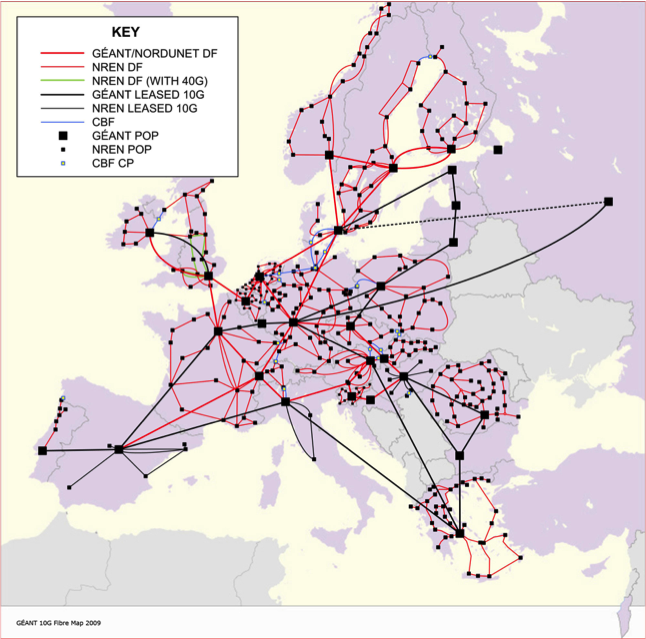
\includegraphics[width=0.46\textwidth]{./figures/geant.png}
\label{fig:geant}
\vspace*{-.35cm}
\caption{The European G\'EANT backbone}
{\small
 G\'EANT is the federation of all European Research and Educational
 Networks.
Each black square corresponds to one network point of presence (\aka.
a PoP) that can host a nano/micro DC.}
\vspace*{-.5cm}
\end{figure}

A preliminary study has established the fundamentals of such an
\emph{in-network distributed cloud} referred by the consortium  as the
\emph{Locality-Based Utility Computing} (LUC) concept
\cite{lebre:beyond2013}. However, the question of how operating such
an infrastructure is still under investigations. Indeed, at this level of
distribution, latency and fault tolerance become primary concerns, and
collaboration between servers of differents location must be organized
wisely.

In this vision paper, we discuss some key-elements that
motivate our choices to design and implement the
\emph{LUC Operating System}, a system in charge of turning
a LUC infrastructure into a collection of abstracted computing
facilities that are as convenient to administrate and use as available
Infrastructure-as-a-Service (IaaS) managers
\cite{cloudstack,opennebula,openstack}.
We explain, in particular, why federated approaches~\cite{buyya:intercloud} are not satisfactory  and
why designing a fully distributed system that operates all resources makes
sense.


%
%
% - Developing from scratch: herculean work.
% - We should maximize the reuse of existing tools/concepts.
% - To do so: 1) draw architectural summary; 2) identify challenges for the
%   LUC-OS 3) instantiate it over OpenStack.
%

%Moreover, we describe the fundamental capabilities the LUC OS should
%deliver.



As the capabilities of the LUC OS  are similar to existing IaaS managers
and because it would be a non-sense technically speaking to develop
the LUC OS from scratch
%considering the number of mechanisms that are
%mandatory to operate a CC infrastructure,
%
we chose to revise the OpenStack solution
\cite{openstack}, leveraging P2P mechanisms. Our current efforts focus
on the validation of a distributed version of the \emph{Nova} service
on top of Grid'5000~\cite{grid5000}. Historically, \emph{Nova} relies
on a MySQL centralized database, preventing it to natively scale
beyond one site. To reach such a goal, we replaced
the MySQL component
by the REDIS backend, a distributed key/value store. Such a modification
enables us to deploy several \emph{Nova} controllers on distinct sites
giving the illusion that there was only one global infrastructure (each
controller
manipulating the \emph{Nova} internal states throughout the REDIS
system).
 This first validation paves
the way toward a complete LUC OS leveraging  the OpenStack ecosystem.


The remaining of the article is as follows: Section
\ref{sec:design} explains our design choices. Section
\ref{sec:leveraging-openstack}
describes the OpenStack and gives first details of our current
Proof-of-Concept.
%A preliminar validation
%of our prototype focusing on the Nova service is presented in Section
%\ref{sec:eval}.
Finally
Section \ref{sec:conclusion}
concludes and discusses future actions.
